\documentclass[onecolumn]{IEEEtran}
\IEEEoverridecommandlockouts
% The preceding line is only needed to identify funding in the first footnote. If that is unneeded, please comment it out.
\usepackage{cite}
\usepackage{amsmath,amssymb,amsfonts}
\usepackage{algorithmic}
\usepackage{graphicx}
\usepackage{textcomp}
\usepackage{xcolor}
\usepackage{amsmath,amsfonts,amsthm,amssymb}
\usepackage{setspace}
\usepackage{Tabbing}
\usepackage{enumitem}
\usepackage{fancyhdr}
\usepackage{lastpage}
\usepackage{extramarks}
\usepackage[hidelinks]{hyperref}
\usepackage{chngpage}
\usepackage{caption}
\usepackage{subcaption}
\usepackage{soul,color}
\usepackage{float}
\usepackage{graphicx,float,wrapfig}
% code listing settings
\usepackage{listings}
\lstset{
    language=Python,
    basicstyle=\ttfamily\small,
    aboveskip={1.0\baselineskip},
    belowskip={1.0\baselineskip},
    columns=fixed,
    extendedchars=true,
    breaklines=true,
    tabsize=4,
    prebreak=\raisebox{0ex}[0ex][0ex]{\ensuremath{\hookleftarrow}},
    frame=lines,
    showtabs=false,
    showspaces=false,
    showstringspaces=false,
    keywordstyle=\color[rgb]{0.627,0.126,0.941},
    commentstyle=\color[rgb]{0.133,0.545,0.133},
    stringstyle=\color[rgb]{01,0,0},
    numbers=left,
    numberstyle=\small,
    stepnumber=1,
    numbersep=10pt,
    captionpos=t,
    escapeinside={\%*}{*)}
}

\def\BibTeX{{\rm B\kern-.05em{\sc i\kern-.025em b}\kern-.08em
    T\kern-.1667em\lower.7ex\hbox{E}\kern-.125emX}}

% Add page numbers
\fancyhf{} % Clear all headers and footers
\fancyfoot[C]{\thepage} % Footer centered with page number
\renewcommand{\headrulewidth}{0pt} % Remove header rule
\renewcommand{\footrulewidth}{0pt} % Remove footer rule

\pagestyle{fancy} % Enable fancy header/footer

\begin{document}

\title{ECE1512 Project A Report}

\author{\IEEEauthorblockN{Rémi Grzeczkowicz} \\
\IEEEauthorblockA{\textit{MScAC Student} \\
\textit{University of Toronto - Department of Computer Science}\\
Student Number: 1010905399\\
remigrz@cs.toronto.edu}
}

\maketitle
\thispagestyle{fancy} % Apply fancy header/footer, including the page number on the first page


% \begin{abstract}
% This document is a model and instructions for \LaTeX.
% This and the IEEEtran.cls file define the components of your paper [title, text, heads, etc.]. *CRITICAL: Do Not Use Symbols, Special Characters, Footnotes, 
% or Math in Paper Title or Abstract.
% \end{abstract}

% \begin{IEEEkeywords}
% component, formatting, style, styling, insert
% \end{IEEEkeywords}

%Table des matières centrée sur une nouvelle page
\vfill
\tableofcontents
\vfill

\newpage

\section{Introduction}
In this report, we will compare two datadistillation method for synthetic dataset generation. The first method is DataDAM \cite{sajedi2023datadam} and the second is PAD \cite{li2024prioritize}. We will use the MNIST and MHIST datasets to generate synthetic datasets and train models on them. We will then compare the performances of the models trained on the synthetic datasets with the models trained on the full datasets. We will also evaluate the synthetic datasets on a cross-architecture setup. Finally, we will use the synthetic datasets to perform a neural architecture search.
The code used for this report is available at \url{https://github.com/jacedoir/ECE1512_2024F_ProjectRepo_Grzeczkowicz}.

\section{Task 1 - DataDAM}
This part relies on the paper \cite{sajedi2023datadam}.

\subsection{Part 1 - Questions anwsering}
\begin{enumerate}[label=(\alph*)]
    \item In this paper, the purpose of using Dataset distillation is to reduce the training cost while preserving the performance of the model.
    \vspace{3mm}
    \item The advantages of their methodology over state-of-the-art are:
    \begin{itemize}
        \item It achieved unbiased representation of the real data distribution.
        \item It does not rely on rely on pre-trained network parameters or employ bi-level optimization.
        \item It has a reduced memory cost with a lower run time thanks to the fact that DataDAM does not use an inner-loop bi-level optimization.
        \item It outperformed other distillation methods except for one case where Matching Training Trajectory (MTT) performed better on CIFAR-10 with 10 Impage Per Class (IPC). MIT got an accuracy of $56.5\% \pm 0.7$ while DataDAM got $54.2\% \pm 0.8$.
    \end{itemize}
    \vspace{3mm}
    \item The novelty provided by this paper is the use of attention in data distillation. Indeed it has been used in knowledge distillation but never in dataset distillation.
    \vspace{3mm}
    \item The methodology is as follows:
    \begin{enumerate}[label=(\arabic*)]
        \item Initialize a synthetic dataset $\mathcal{S}$ either using random noise or sampling from the original training dataset $\mathcal{T}$.
        \item For each class $k$ a batch $B_T^k$ of real images and a batch $B_S^k$ of synthetic images are sampled from $\mathcal{T}$ and $\mathcal{S}$ respectively.
        \item Then a neural network $\phi_\theta$ is employed to extract features from the images. The network have different layers, each creating a feature map. This multiple feature maps allow to capture low-level, mid-level and high-level representations of the data.
        \item Using the feature maps of each layer, the Spatial Attention Matching (SAM) module generates an attention map for real and synthetic images. The attention map is formulated as $A(f_{\theta,l}^{T_k}) = \sum_{i=1}^{C_l} | (f_{\theta,l}^{T_k})_i|^p$ where $(f_{\theta,l}^{T_k})_i$ is the $i$-th feature map in the $l$th layer, $C_l$ is the number of channels and $p$ is a parameter to adjust the weights of the feature maps.
        \item The attention maps for both datasets are then compared using the loss function $\mathcal{L}_{SAM}$.
        \item The output of the network for each dataset is also compared using the loss function $\mathcal{L}_{MMD}$ based on the Maximum Mean Discrepancy (MMD).
        \item The total loss is then given by $\mathcal{L} = \mathcal{L}_{SAM} + \mathcal{L}_{MMD}$.
        \item Then $\mathcal{S}$ is updated such as $\mathcal{S} = arg \min_{\mathcal{S}} \mathcal{L}$.
    \end{enumerate}
    \vspace{3mm}
    \item DataDAM could be used in machine learning for continual learning by providing an efficient memory management method by storing the synthetic data in the memory instead of the real data. This allows for a better memory usage and a lower computational cost. DataDAM could also be used for neural architecture search. Indeed, instead of training many architectures on the full dataset, those architectures could trained on the distilled dataset, leading to a faster search.
\end{enumerate}

\subsection{Part 2 - Data Distillation Learning using DataDAM}
\subsubsection{Build the distillation model}
To build the distillation model, we used the code provided by the author of \cite{sajedi2023datadam} in the repo \cite{githubGitHubDataDistillationDataDAM}. This allowed us to create a DataDAM class that we could use. Some change were required to make the understanding easier and to fit our framework as well as remove the unneeded parts. The code is provided in the annex \ref{sec:DataDAM_code}.
\\
In \cite{githubGitHubDataDistillationDataDAM}, we can notice that the authors introduced a factor $100$ in their loss. After various attempt, and because they use more iterations than we do, we decided to set the factor to $10 000$ so that the loss is not too small and the dataset is updated correctly.
\\
\subsubsection{Distillation of MNIST dataset from real data}
To generate the synthetic dataset associated with the MNIST dataset, we used the DataDAM class. The parameters used were : $model = ConvNet3D$, $IPC = 10$, $K=100$, $T=10$, $\eta_S = 0.1$, $\zeta_S = 1$, $\eta_\theta = 0.01$, $\zeta_\theta=50$, $\lambda_{mmd}=0.01$ and $minibatches_{size}=256$.
\begin{figure}[H]
    \centering
    \begin{subfigure}{.5\textwidth}
        \centering
        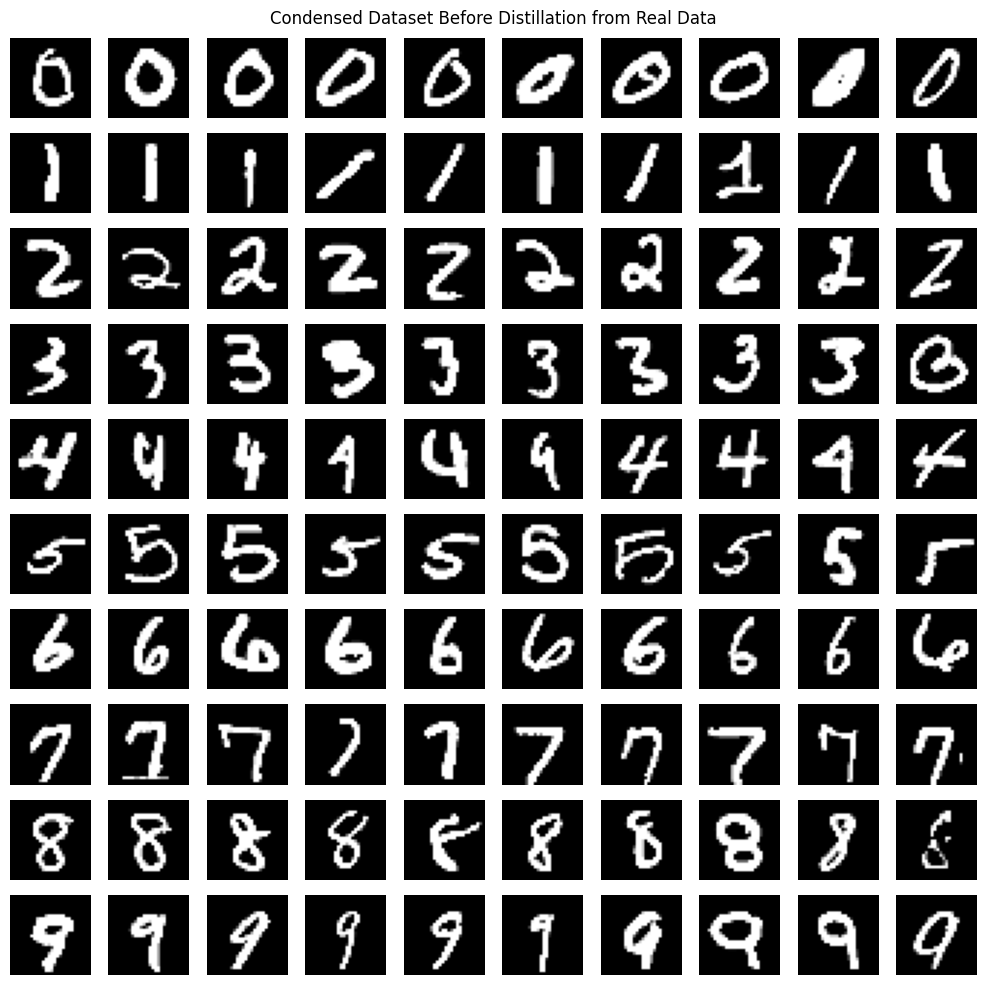
\includegraphics[width=0.95\textwidth]{images/MNIST_datadam_before_distil_real.png}
        \caption{The synthetic dataset before distillation from real data}
        \label{fig:MNIST_datadam_before_distil_real}
    \end{subfigure}%
    \begin{subfigure}{.5\textwidth}
        \centering
        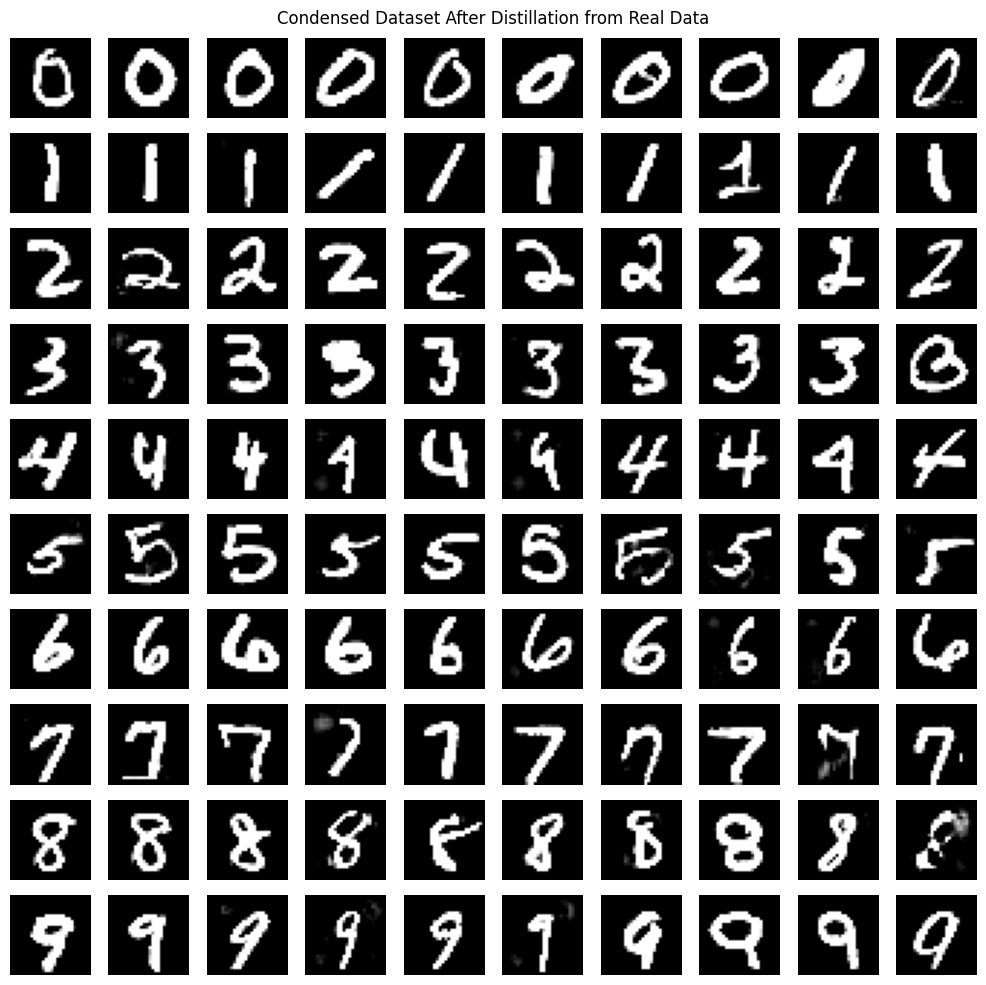
\includegraphics[width=0.95\textwidth]{images/MNIST_datadam_after_distil_real.png}
        \caption{The synthetic dataset after distillation from real data}
        \label{fig:MNIST_datadam_after_distil_real}
    \end{subfigure}
    \caption{The synthetic dataset before and after distillation from real data}
\end{figure}
% \begin{figure}[H]
%     \centering
%     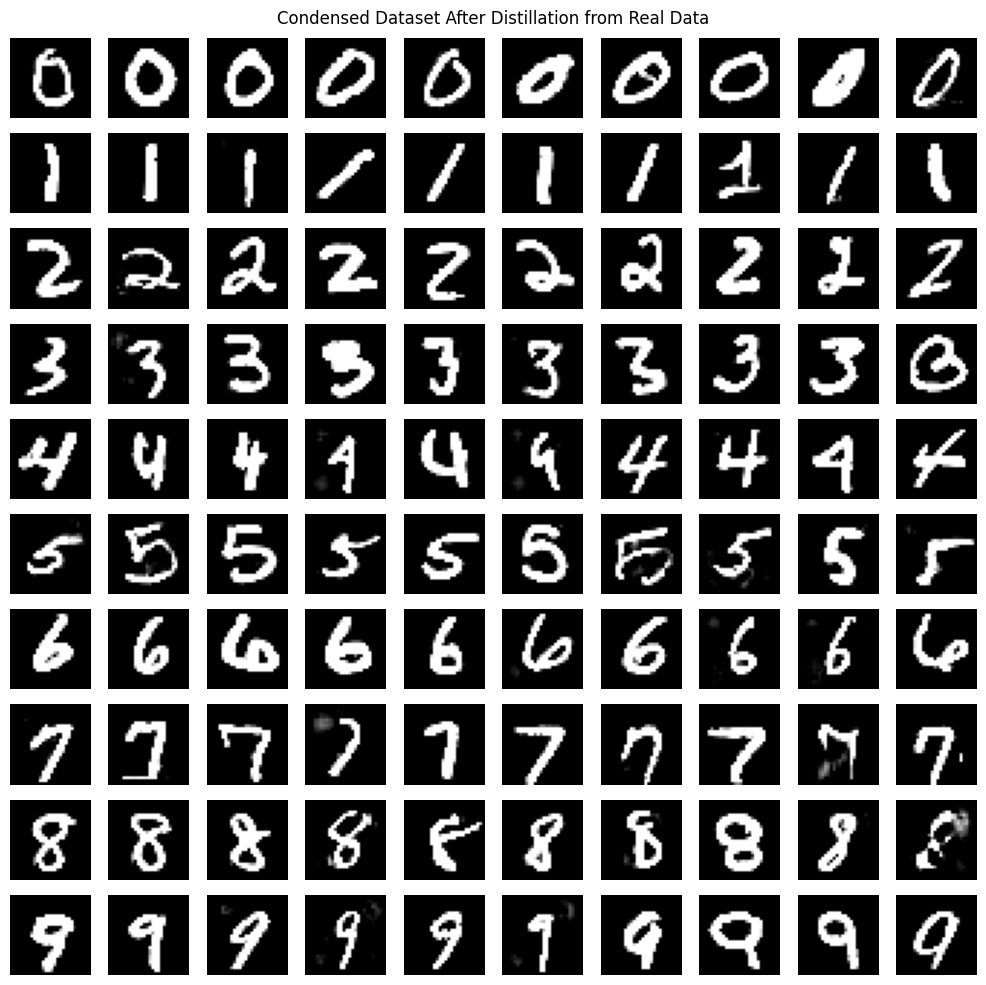
\includegraphics[width=0.5\textwidth]{images/MNIST_datadam_after_distil_real.png}
%     \caption{The synthetic dataset after distillation from real data}
%     \label{fig:MNIST_datadam_after_distil_real}
% \end{figure}


Figure \ref{fig:MNIST_datadam_before_distil_real} presents the synthetic dataset prior to distillation from real data, while Figure \ref{fig:MNIST_datadam_after_distil_real} illustrates the dataset following distillation. At first glance, the synthetic dataset closely resembles the real dataset. To gain deeper insight into the differences between them, we can refer to Figure \ref{fig:MNIST_diff_real}, which highlights the distinctions between the synthetic dataset before and after distillation. Notably, these differences are subtle, mainly reflecting variations in the finer details of digit shapes. This observation suggests that the synthetic dataset effectively encapsulates the key information from the real dataset.

\begin{figure}[H]
    \centering
    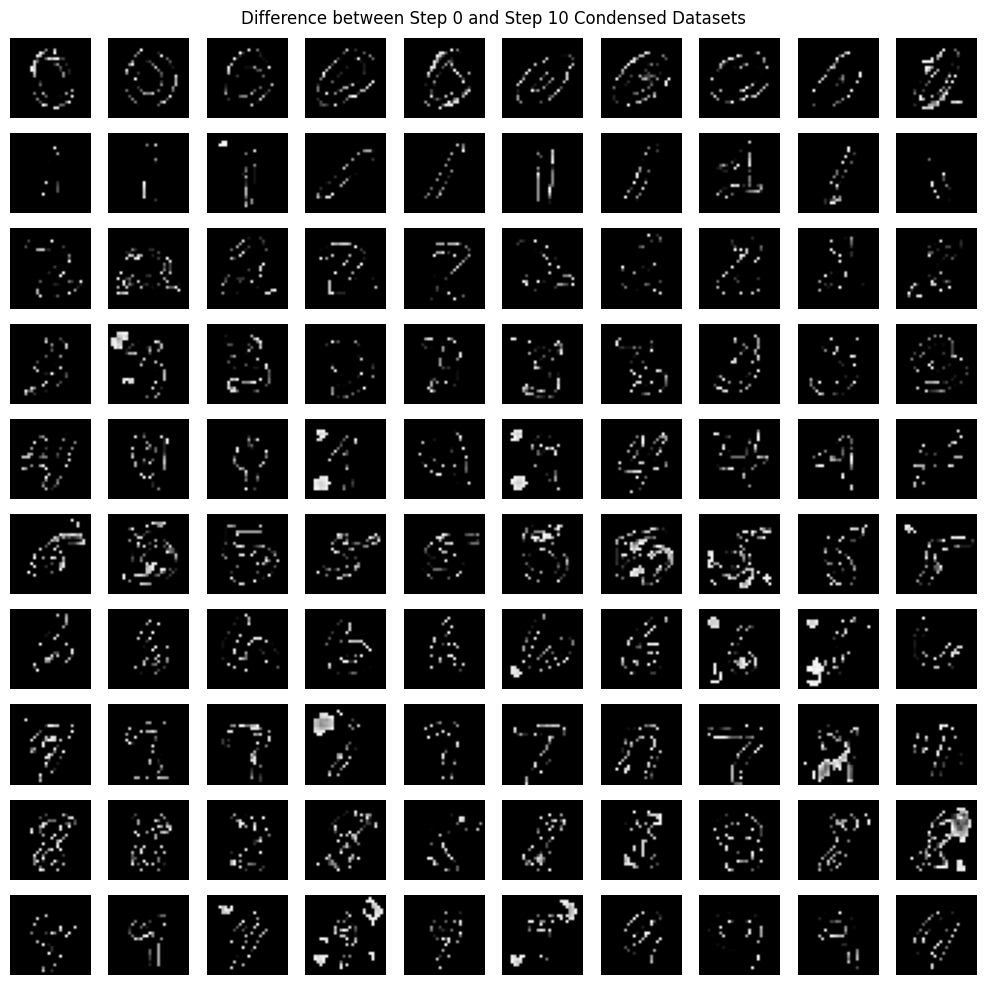
\includegraphics[width=0.5\textwidth]{images/MNIST_diff_real.png}
    \caption{The difference between the synthetic dataset before and after distillation from real data}
    \label{fig:MNIST_diff_real}
\end{figure}

\subsubsection{Distillation of MNIST dataset from gaussian noise}
To generate the gaussin noise, we used a standard normal distribution. The parameters used were the same as for the distillation from real data.

\begin{figure}[H]
    \centering
    \begin{subfigure}{.5\textwidth}
        \centering
        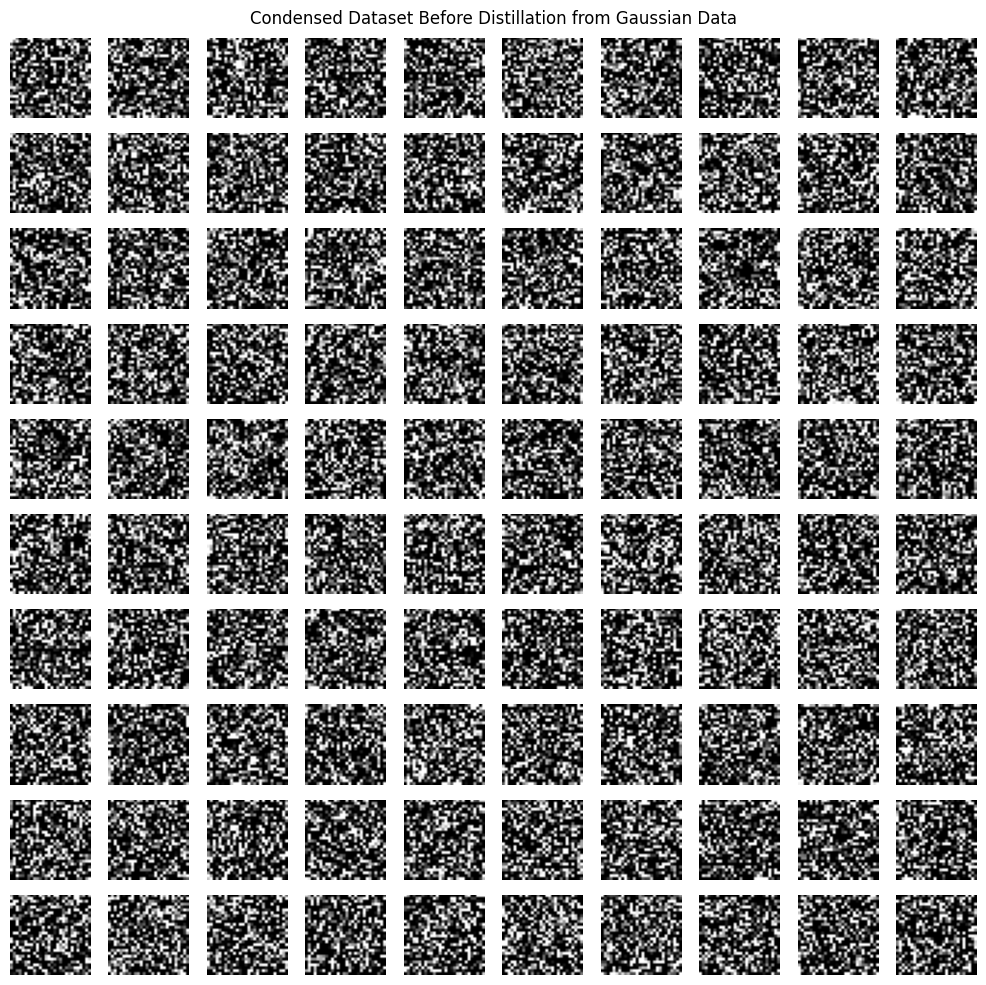
\includegraphics[width=0.95\textwidth]{images/MNIST_datadam_before_distil_gaussian.png}
        \caption{The synthetic dataset before distillation from gaussian noise}
        \label{fig:MNIST_datadam_before_distil_gaussian}
    \end{subfigure}%
    \begin{subfigure}{.5\textwidth}
        \centering
        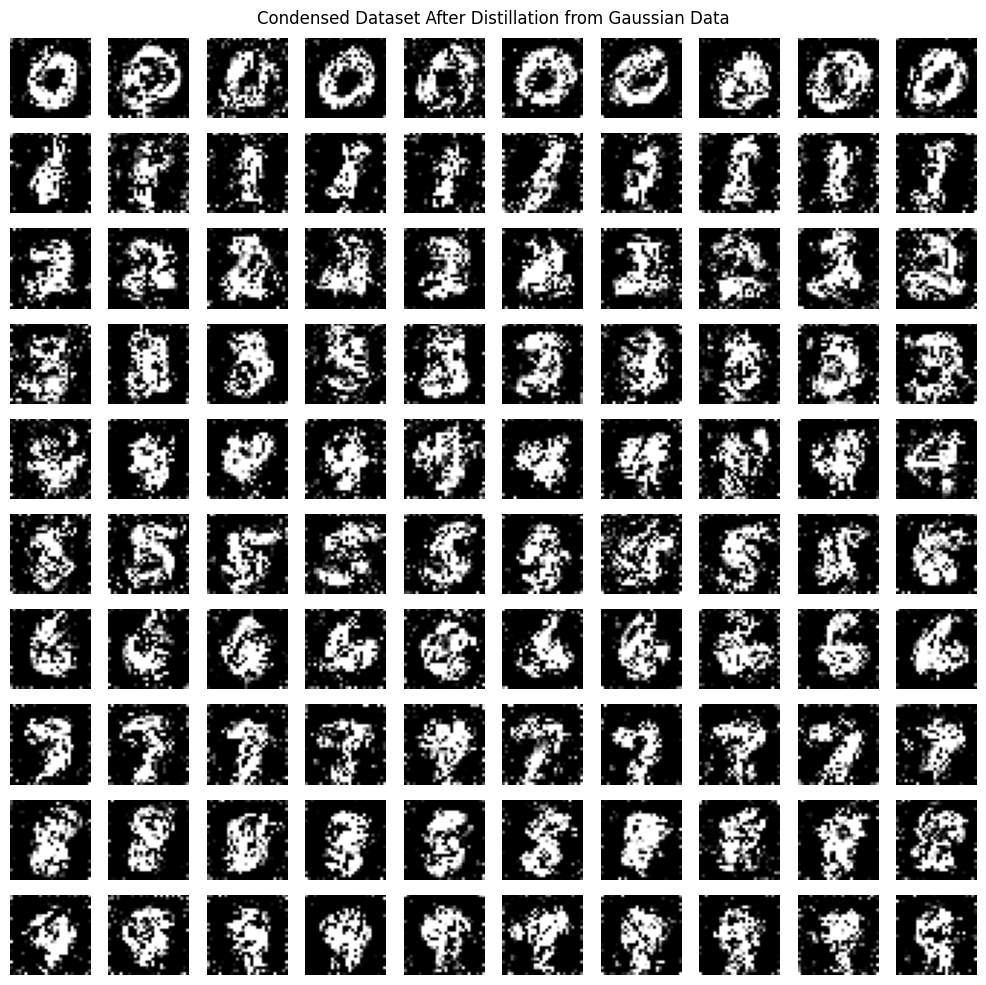
\includegraphics[width=0.95\textwidth]{images/MNIST_datadam_after_distil_gaussian.png}
        \caption{The synthetic dataset after distillation from gaussian noise}
        \label{fig:MNIST_datadam_after_distil_gaussian}
    \end{subfigure}
    \caption{The synthetic dataset before and after distillation from gaussian noise}
\end{figure}

Figure \ref{fig:MNIST_datadam_before_distil_gaussian} shows the synthetic dataset generated before distillation from Gaussian noise, and Figure \ref{fig:MNIST_datadam_after_distil_gaussian} displays the dataset after distillation. The distillation process successfully produced a synthetic dataset with recognizable digit shapes. However, the quality of these digits remains low.
\\
\subsubsection{Resutls and discussion for the MNIST dataset}
We then trained a ConvNet3D model for 50 epochs on the full MNIST dataset and on the two synthetic datasets. The results are shown in Table \ref{tab:MNIST_results}.

\begin{table}[H]
    \centering
    \begin{tabular}{|c|c|c|c|}
        \hline
        Dataset & Full & From gaussian & From real \\
        \hline
        Accuracy & $99.49\%$ & $74.44\%$ & $91.81\%$ \\
        \hline
        Training Time & 7 min 7 s & $<$ 1 s & $<$ 1 s \\
        \hline
    \end{tabular}
    \caption{Results for the MNIST dataset}
    \label{tab:MNIST_results}
\end{table}

The model trained on the real dataset achieved the highest accuracy; however, its training time was significantly longer compared to the models trained on the synthetic datasets. The model trained on the synthetic dataset generated from Gaussian noise performed the worst, as expected, given the low quality of that dataset. In contrast, the model trained on the synthetic dataset distilled from real data achieved good accuracy with a considerably shorter training time than the model trained on the full dataset, indicating the efficiency of the distillation method in reducing training time while preserving model performance.
\\
\\
We further evaluated the datasets in a cross-architecture setup by training AlexNet on both the full MNIST dataset and the two synthetic datasets. The results, shown in Table \ref{tab:MNIST_results_cross_architecture}, reveal that AlexNet performs poorly on the synthetic datasets. This discrepancy may be due to the fact that the synthetic dataset was generated using a ConvNet3D model, making it difficult for AlexNet to capture the same information.

\begin{table}[H]
    \centering
    \begin{tabular}{|c|c|c|c|}
        \hline
        Dataset & Full & From gaussian & From real \\
        \hline
        Accuracy & $99.19\%$ & $17.9\%$ & $23.48\%$ \\
        \hline
        Training Time & 9 min 22 s & $<$ 1 s & $<$ 1 s \\
        \hline
    \end{tabular}
    \caption{Results for the MNIST dataset on cross-architecture setup (AlexNet)}
    \label{tab:MNIST_results_cross_architecture}
\end{table}

\subsubsection{Distillation of the MHIST dataset from real data}
To generate the synthetic dataset associated with the MHIST dataset, we used the DataDAM class. The parameters used were : $model = ConvNet7D$, $IPC = 50$, $K=200$, $T=10$, $\eta_S = 100$, $\zeta_S = 1$, $\eta_\theta = 0.01$, $\zeta_\theta=50$, $\lambda_{mmd}=0.01$ and $minibatches_{size}=128$.

\begin{figure}[H]
    \centering
    \begin{subfigure}{.5\textwidth}
        \centering
        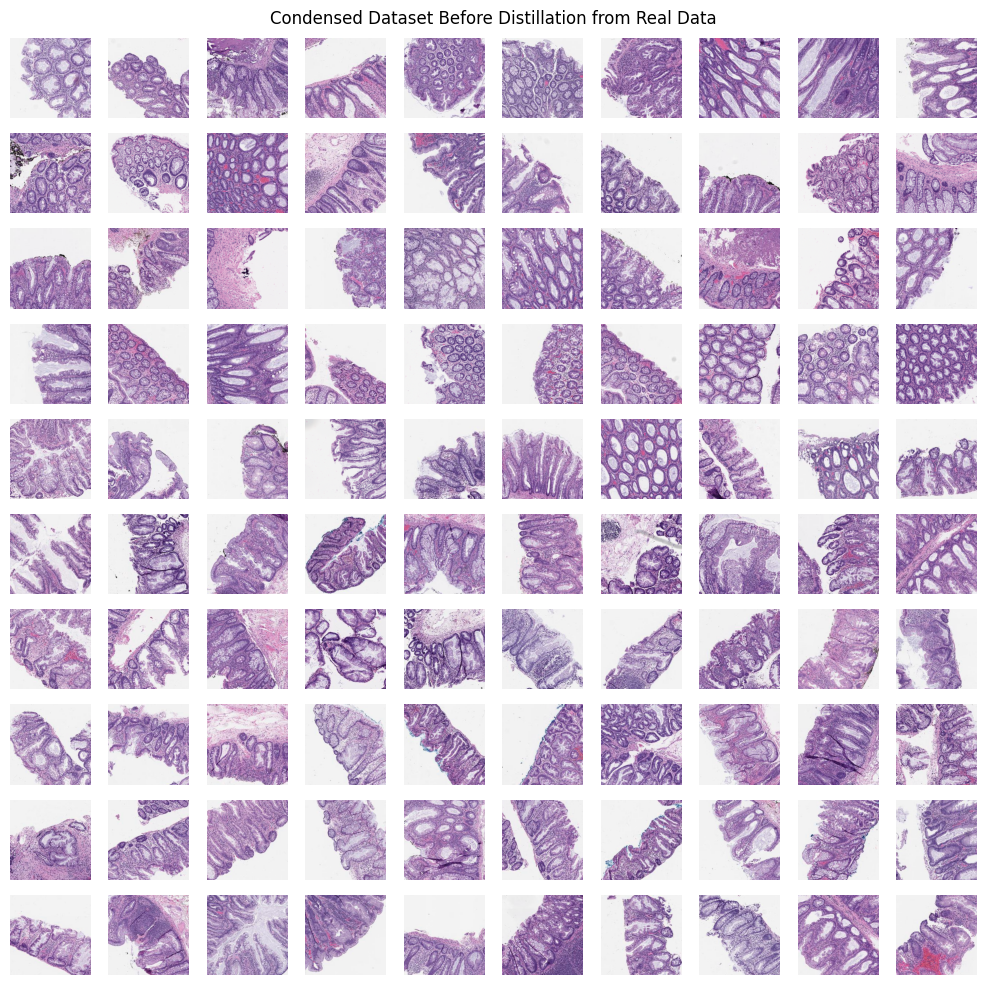
\includegraphics[width=0.95\textwidth]{images/MHIST_datadam_before_distil_real.png}
        \caption{The synthetic dataset before distillation from real data}
        \label{fig:MHIST_datadam_before_distil_real}
    \end{subfigure}%
    \begin{subfigure}{.5\textwidth}
        \centering
        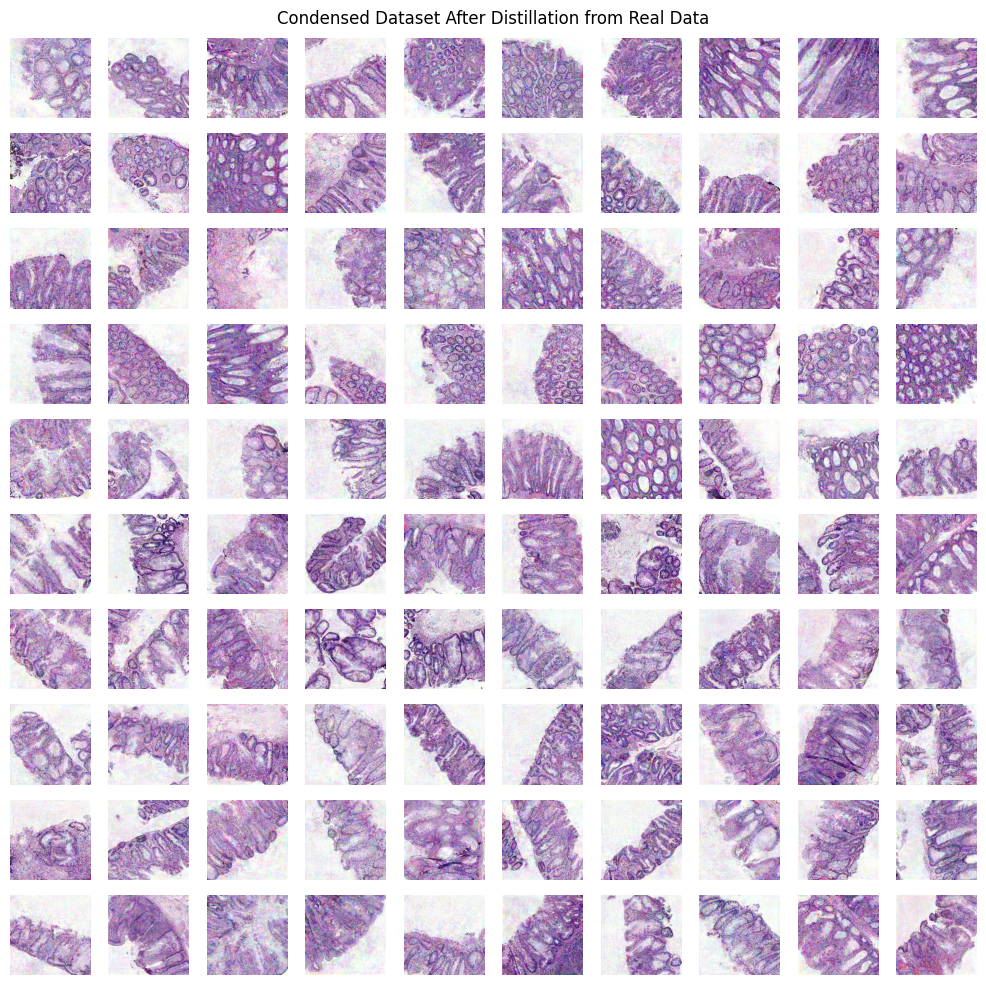
\includegraphics[width=0.95\textwidth]{images/MHIST_datadam_after_distil_real.png}
        \caption{The synthetic dataset after distillation from real data}
        \label{fig:MHIST_datadam_after_distil_real}
    \end{subfigure}
    \caption{The synthetic dataset before and after distillation from real data}
\end{figure}

Figure \ref{fig:MHIST_datadam_before_distil_real} displays the synthetic dataset before distillation from real data, while Figure \ref{fig:MHIST_datadam_after_distil_real} shows the dataset after distillation. At first glance, the synthetic dataset appears nearly identical to the real dataset, with the main differences observed in the image backgrounds. For a clearer comparison, Figure \ref{fig:MHIST_diff_real} highlights the differences between the synthetic dataset before and after distillation. This figure shows that the entire image undergoes updates during distillation, indicating that the synthetic dataset is not a simple copy of the real dataset.

\begin{figure}[H]
    \centering
    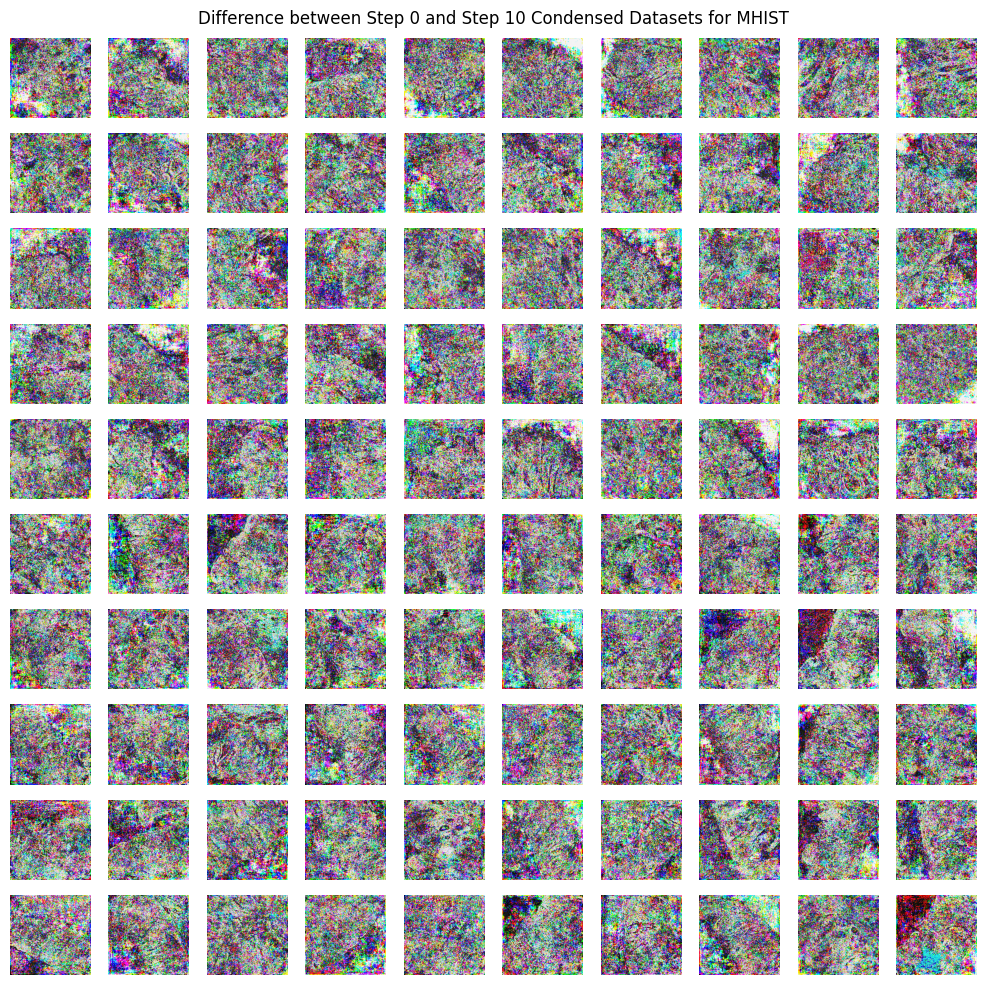
\includegraphics[width=0.5\textwidth]{images/MHIST_diff_real.png}
    \caption{The difference between the synthetic dataset before and after distillation from real data}
    \label{fig:MHIST_diff_real}
\end{figure}

\subsubsection{Distillation of the MHIST dataset from gaussian noise}
To generate the gaussin noise, we used a standard normal distribution. The parameters used were the same as for the distillation from real data.

\begin{figure}[H]
    \centering
    \begin{subfigure}{.5\textwidth}
        \centering
        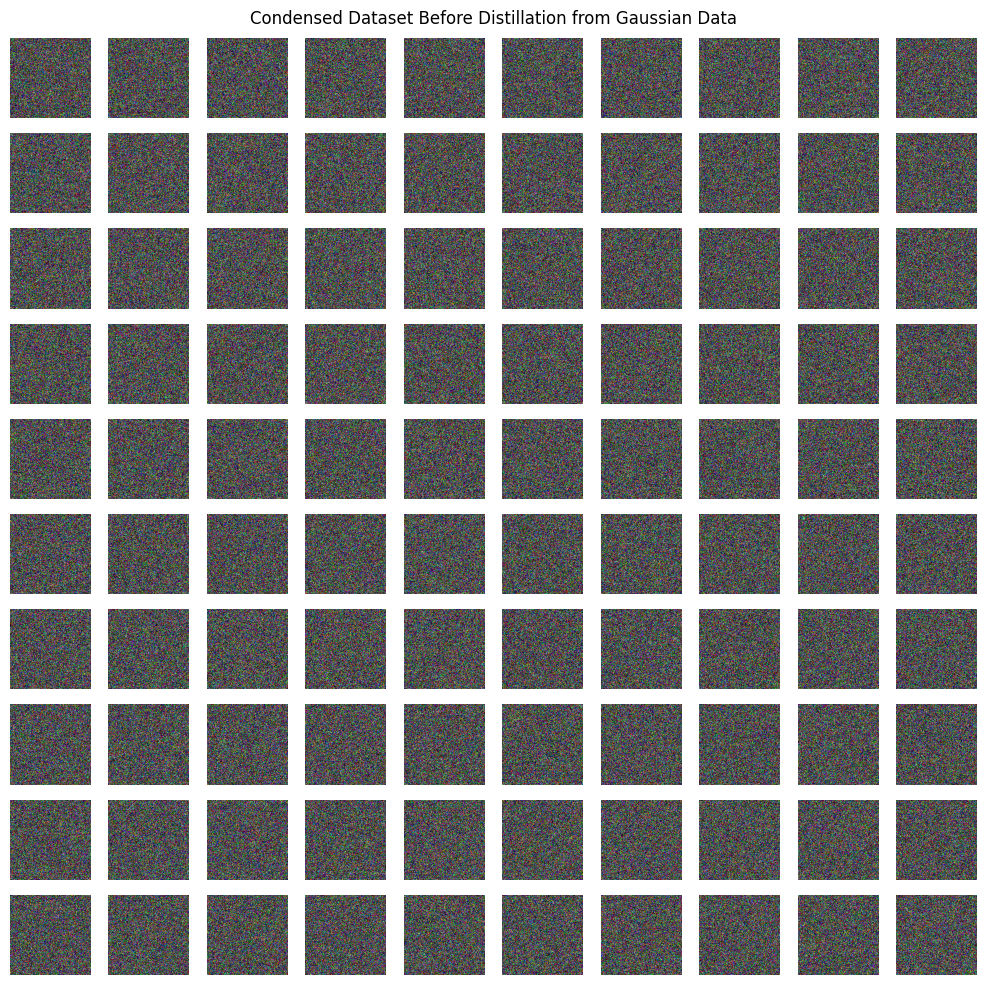
\includegraphics[width=0.95\textwidth]{images/MHIST_datadam_before_distil_gaussian.png}
        \caption{The synthetic dataset before distillation from gaussian noise}
        \label{fig:MHIST_datadam_before_distil_gaussian}
    \end{subfigure}%
    \begin{subfigure}{.5\textwidth}
        \centering
        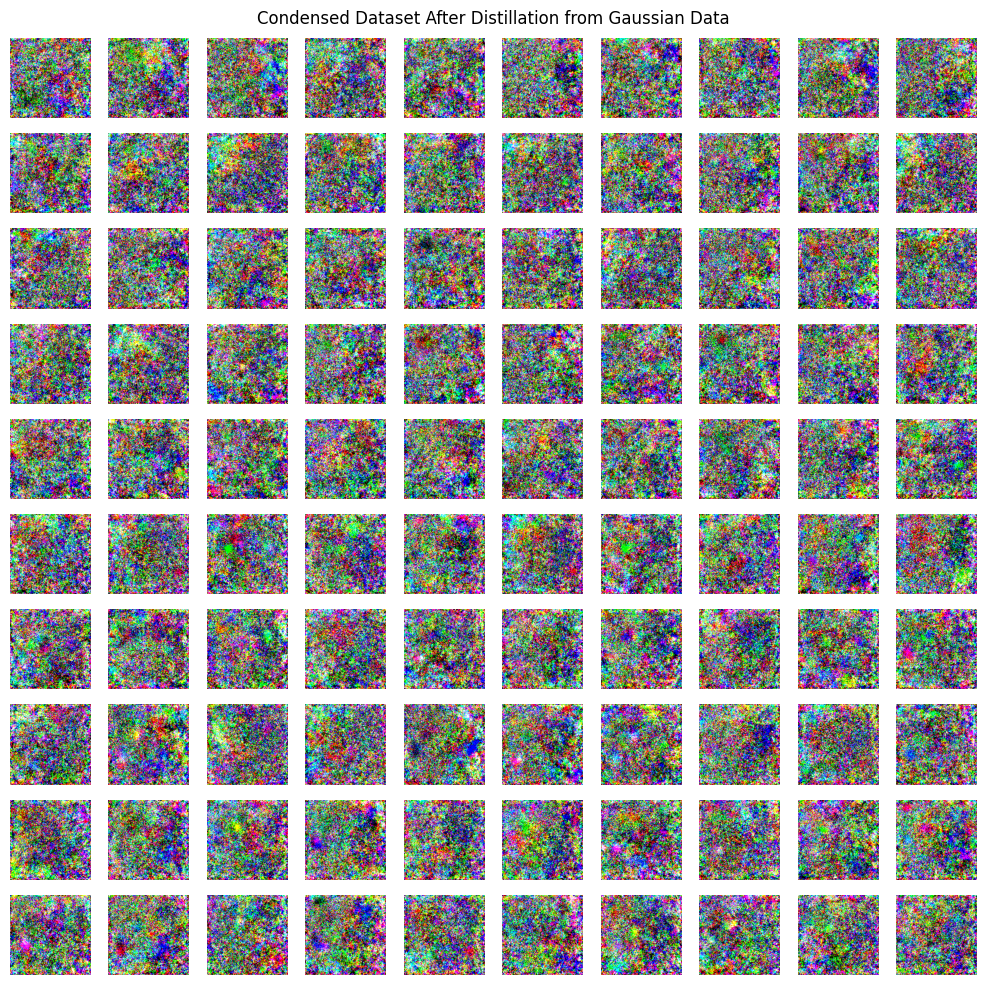
\includegraphics[width=0.95\textwidth]{images/MHIST_datadam_after_distil_gaussian.png}
        \caption{The synthetic dataset after distillation from gaussian noise}
        \label{fig:MHIST_datadam_after_distil_gaussian}
    \end{subfigure}
    \caption{The synthetic dataset before and after distillation from gaussian noise}
\end{figure}

Figure \ref{fig:MHIST_datadam_before_distil_gaussian} shows the synthetic dataset before distillation from Gaussian noise, while Figure \ref{fig:MHIST_datadam_after_distil_gaussian} displays the dataset after distillation. Unlike the MNIST dataset, the synthetic dataset generated from Gaussian noise for MHIST is not recognizable. This result is expected due to the increased complexity of the data, which includes three color channels as well as more intricate image content.

\subsubsection{Resutls and discussion for the MHIST dataset}
\label{sec:MHIST_results}
We then trained a ConvNet7D model for 50 epochs on the full MHIST dataset and on the two synthetic datasets. The results are shown in Table \ref{tab:MHIST_results}.

\begin{table}[H]
    \centering
    \begin{tabular}{|c|c|c|c|}
        \hline
        Dataset & Full & From gaussian & From real \\
        \hline
        Accuracy & $80.14\%$ & $53.63\%$ & $63.87\%$ \\
        \hline
        Training Time & 6 min 12 s & 10 s & 10 s \\
        \hline
    \end{tabular}
    \caption{Results for the MHIST dataset}
    \label{tab:MHIST_results}
\end{table}

The model trained on the real dataset achieves the highest accuracy, though its training time is significantly longer than that of models trained on synthetic datasets. The model trained on the synthetic dataset generated from Gaussian noise performs the worst, with accuracy close to random guessing. By contrast, the model trained on the synthetic dataset distilled from real data achieves better accuracy with a shorter training time, demonstrating that the distillation method effectively reduces training time, albeit with some loss of accuracy—expected, as the synthetic dataset is not a perfect replica of the real dataset.

Next, we evaluate the datasets in a cross-architecture setup by training AlexNet on both the full MHIST dataset and the two synthetic datasets, with results shown in Table \ref{tab:MHIST_results_cross_architecture}. Surprisingly, the model trained on the synthetic dataset distilled from real data shows lower accuracy than the model trained on the synthetic dataset from Gaussian noise, with the latter achieving nearly comparable performance to the model trained on the full dataset. This could be because the synthetic dataset distilled from real data may be too well-suited to the ConvNet7D model, while the Gaussian noise synthetic dataset’s lower fidelity encourages better generalization across different architectures.

\begin{table}[H]
    \centering
    \begin{tabular}{|c|c|c|c|}
        \hline
        Dataset & Full & From gaussian & From real \\
        \hline
        Accuracy & $68.37\%$ & $63.15\%$ & $36.87\%$ \\
        \hline
        Training Time & 6 min 40 s & 17 s & 18 s \\
        \hline
    \end{tabular}
    \caption{Results for the MHIST dataset on cross-architecture setup (AlexNet)}
    \label{tab:MHIST_results_cross_architecture}
\end{table}

\subsubsection{Neural architecture search}
We then propose using the synthetic dataset to perform a neural architecture search to identify the optimal ConvNet model for classifying either the MNIST or MHIST datasets. The search will include the following models: ConvNetD1, ConvNetD2, ConvNetD3, ConvNetD4, ConvNetD5, ConvNetW32, ConvNetW64, ConvNetW128, ConvNetW256, ConvNetAS, ConvNetAR, ConvNetAL, ConvNetASwish, ConvNetASwishBN, ConvNetNN, ConvNetBN, ConvNetLN, ConvNetIN, ConvNetGN, ConvNetNP, ConvNetMP, and ConvNetAP.
\\
Results for the MNIST dataset are presented in Table \ref{tab:NAS_results_MNIST}. We observe that using the synthetic dataset for architecture search is significantly faster than training the best architecture directly on the full dataset. In both approaches, the best model achieves high accuracy on the full dataset, demonstrating the effectiveness of the synthetic dataset in conducting a neural architecture search.

\begin{table}[H]
    \centering
    \begin{tabular}{|c|c|c|c|}
        \hline
        Search & From Real & From Gaussian \\
        \hline
        Best Model & ConvNetW256 & ConvNetW64\\
        \hline
        Accuracy on best model trained with synthetic data & $91.92\%$ & $75.79\%$ \\
        \hline
        Research time & 34 s & 82.83 s \\
        \hline
        Accuracy on best model trained on full data & $99.52\%$ & $99.5\%$ \\
        \hline
        Training time on full data & 8 min 4 s & 7 min 27 s \\
        \hline
    \end{tabular}
    \caption{Results for the MNIST dataset}
    \label{tab:NAS_results_MNIST}
\end{table}

For the MHIST dataset, the results are shown in Table \ref{tab:NAS_results_MHIST}. We observe that searching for the best architecture using the synthetic dataset is much faster than training the best architecture directly on the full dataset. However, the model identified through the neural architecture search does not perform as well as the model trained on the full dataset, as discussed in Section \ref{sec:MHIST_results}. This discrepancy may arise because, unlike the MNIST dataset, the synthetic dataset for MHIST does not yield strong performance. Consequently, using it for neural architecture search may propagate the inherent errors of the synthetic dataset, leading to less effective model selection.

\begin{table}[H]
    \centering
    \begin{tabular}{|c|c|c|c|}
        \hline
        Search & From Real & From Gaussian \\
        \hline
        Best Model & ConvNetGN & ConvNetAS\\
        \hline
        Accuracy on best model trained with synthetic data & $64.79\%$ & $63.15\%$ \\
        \hline
        Research time & 10 min 56 s & 10 min 55 s \\
        \hline
        Accuracy on best model trained on full data & $67.04\%$ & $63.66\%$ \\
        \hline
        Training time on full data & 3 min 45 s & 3 min 36 s \\
        \hline
    \end{tabular}
    \caption{Results for the MHIST dataset}
    \label{tab:NAS_results_MHIST}
\end{table}

\section{Task 2 - PAD}
This part relies on the paper \cite{li2024prioritize}.
\subsection{Part 1 - Questions anwsering}
\begin{enumerate}[label=(\alph*)]
    \item The PAD method wants to solve the problem of misaligned information whether extracted or embedded into the synthetic dataset. The goal is to une only high-quality informations to improve the synthetic dataset.
    \vspace{3mm}
    \item PAD introduced two novelties. The first one is the filtering of misaligned information during the extraction step by chosing the data to use according to the difficulty of samples and the image per class ration. The second novelty is the use of a layer-wise filtering in embedding. PAD only uses the deep layers of the agent model to perform distillation as they tend to captures higher quality information.
    \vspace{3mm}
    \item The methodology is as follows:
    \begin{enumerate}[label=(\arabic*)]
        \item The real dataset is scored using a difficulty scoring function $\chi_t(x, y) = \mathbb{E} \left\| p(w_t, x) - y \right\|_2$ where $x$ is a data point, $y$ its label and $p(w_t,x)=\sigma(f(w_t, x))$ is the output of a model $f$ transformed into a probability distribution.
        \item Using this difficulty score, a data scheduler is define as follow. All the easy data are selected first, then the hard data is gradually added to the set following the order of difficulty. When all the data is in the set, the easy data is gradually removed.
        \item An agent model is trained on the real dataset $\mathcal{D}_R$ using a Trajectory-Matching based method and the scheduler described. Then the change of parameters are stored. Let $\{\theta_t^*\}_0^N$ be a parameter sequence of the agent model (it is also called the trajectory). 
        \item At each ineration, $\theta_t^*$ and $\theta_{t+M}^*$ are selected as start and target parameters. Let $\hat\theta_t$ be the parameters of the student agent model trained on the synthetic dataset $\mathcal{D}_S$. Then for $N$ steps $\hat\theta_{t+i+1} = \hat\theta_{t+i} + \alpha \nabla\mathcal{L}_{CE}(\hat\theta_{t+i}, \mathcal{D}_S)$ where $\mathcal{L}_{CE}$ is the cross-entropy loss.
        \item To filter information $\hat\theta_{t+N}$ is defined such as only the $L-k$ last layers are used for matching where $k=\alpha*L$ and $\alpha$ is a hyperparameter that should be low in case of small IPC and high in case of high IPC.
        \item Then the synthetic dataset is updated such as it minimizes $\mathcal{L}$ where $\mathcal{L}=\frac{\left\|\hat\theta_{t+N}-\theta^*_{t+M}\right\|}{\left\|\theta^*_{t+M}-\theta^*_t\right\|}$.
    \end{enumerate}
    \vspace{3mm}
    \item The advantages of PAD are: an improved alignment of information, a high-level of information (by discarding shallow layers) and, according to the paper, a better performance than other methods. The desadvanteges are the introduction of hyperparameter (notably $\alpha$) that have to be tuned, the dependence of the difficulty scoring function that could be hard to define/improve. I believe that this method could distill the dataset correctly accordingt to the performances authors got. I believe that PAD will have more trouble with large scale dataset as the difficulty scoring function may score the entire dataset as difficult and thus leading to a non optimal scheduler.
\end{enumerate}

\subsection{Part 2 - Data Distillation Learning using PAD}
\subsubsection{Build the distillation model}
To build the distillation model, we used the code provided by the author of \cite{li2024prioritize} in the repo \cite{githubGitHubNUSHPCAILabPAD}. This allowed us to create a PAD class that we could use. As previously, some change were required to make the understanding easier and to fit our framework as well as remove the unneeded parts. The code is provided in the annex \ref{sec:PAD_code}.

\subsubsection{Distillation of MNIST dataset from real data}
To generate the synthetic dataset associated with the MNIST dataset, we used the PAD class. The parameters used were : $model = ConvNet3D$, $IPC = 10$, $K=100$, $T=10$, $\eta_S = 1$, $\zeta_S = 1$, $\eta_\theta = 0.01$, $\zeta_\theta=50$ and $\alpha=0.5$ (we take the data from all the layer as they are too few in ConvNet3D).

\begin{figure}[H]
    \centering
    \begin{subfigure}{.5\textwidth}
        \centering
        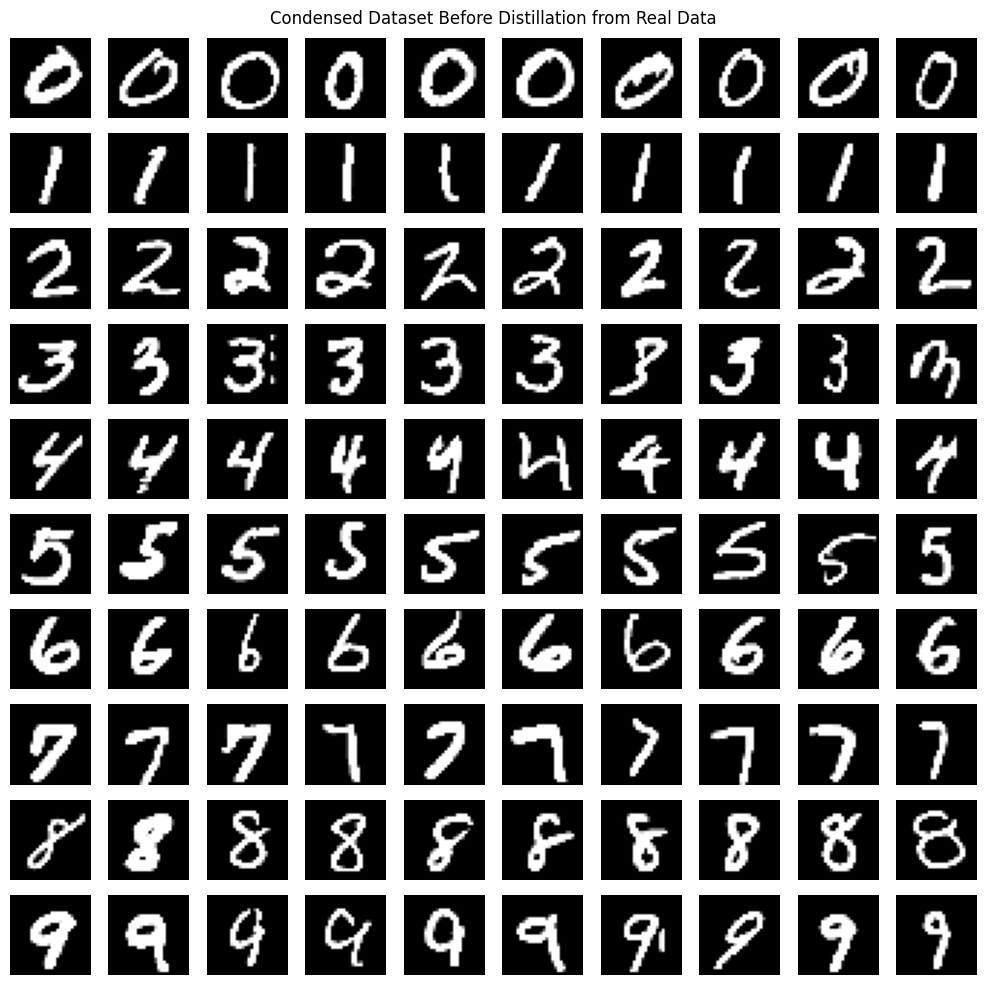
\includegraphics[width=0.95\textwidth]{images/MNIST_pad_before_distil_real.png}
        \caption{The synthetic dataset before distillation from real data}
        \label{fig:MNIST_pad_before_distil_real}
    \end{subfigure}%
    \begin{subfigure}{.5\textwidth}
        \centering
        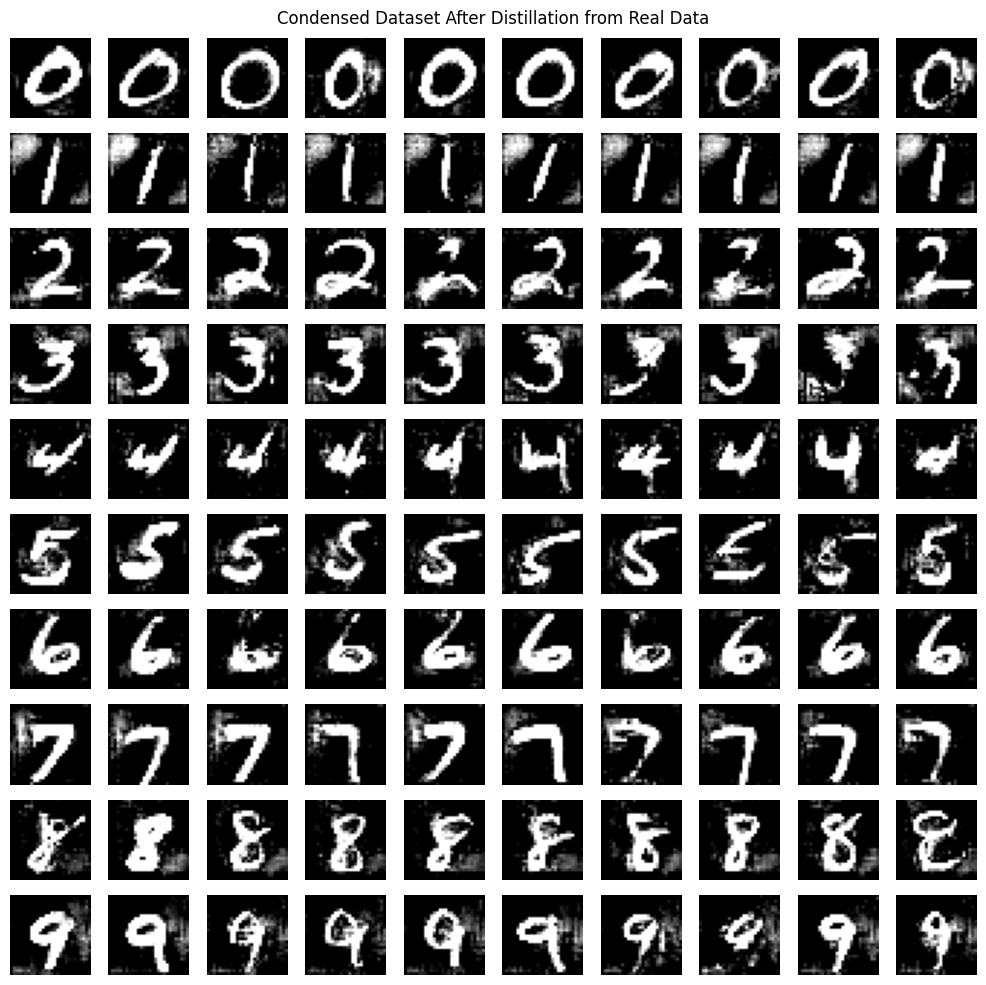
\includegraphics[width=0.95\textwidth]{images/MNIST_pad_after_distil_real.png}
        \caption{The synthetic dataset after distillation from real data}
        \label{fig:MNIST_pad_after_distil_real}
    \end{subfigure}
    \caption{The synthetic dataset before and after distillation from real data}
\end{figure}

Figure \ref{fig:MNIST_pad_before_distil_real} presents the synthetic dataset before distillation from real data, while Figure \ref{fig:MNIST_pad_after_distil_real} displays the dataset after distillation. At first glance, the synthetic dataset appears nearly identical to the real dataset. For a clearer comparison, we can examine Figure \ref{fig:MNIST_2_diff_real}, which illustrates the differences between the synthetic dataset before and after distillation. The differences primarily lie in the finer details of the digit shapes. This is encouraging, as it indicates that the synthetic dataset effectively condenses the essential information from the real dataset.

\begin{figure}[H]
    \centering
    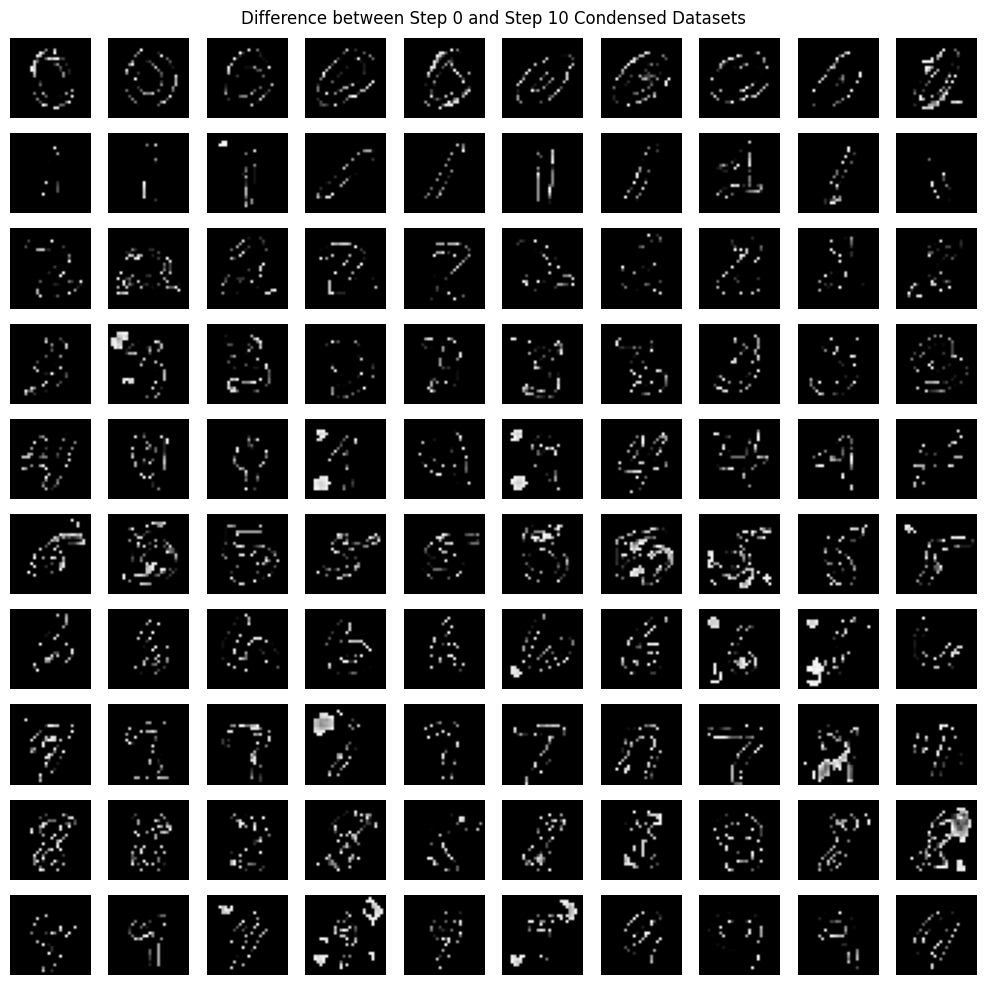
\includegraphics[width=0.5\textwidth]{images/MNIST_2_diff_real.png}
    \caption{The difference between the synthetic dataset before and after distillation from real data}
    \label{fig:MNIST_2_diff_real}
\end{figure}

\subsubsection{Distillation of MNIST dataset from gaussian noise}
To generate the gaussin noise, we used a standard normal distribution. The parameters used were the same as for the distillation from real data.

\begin{figure}[H]
    \centering
    \begin{subfigure}{.5\textwidth}
        \centering
        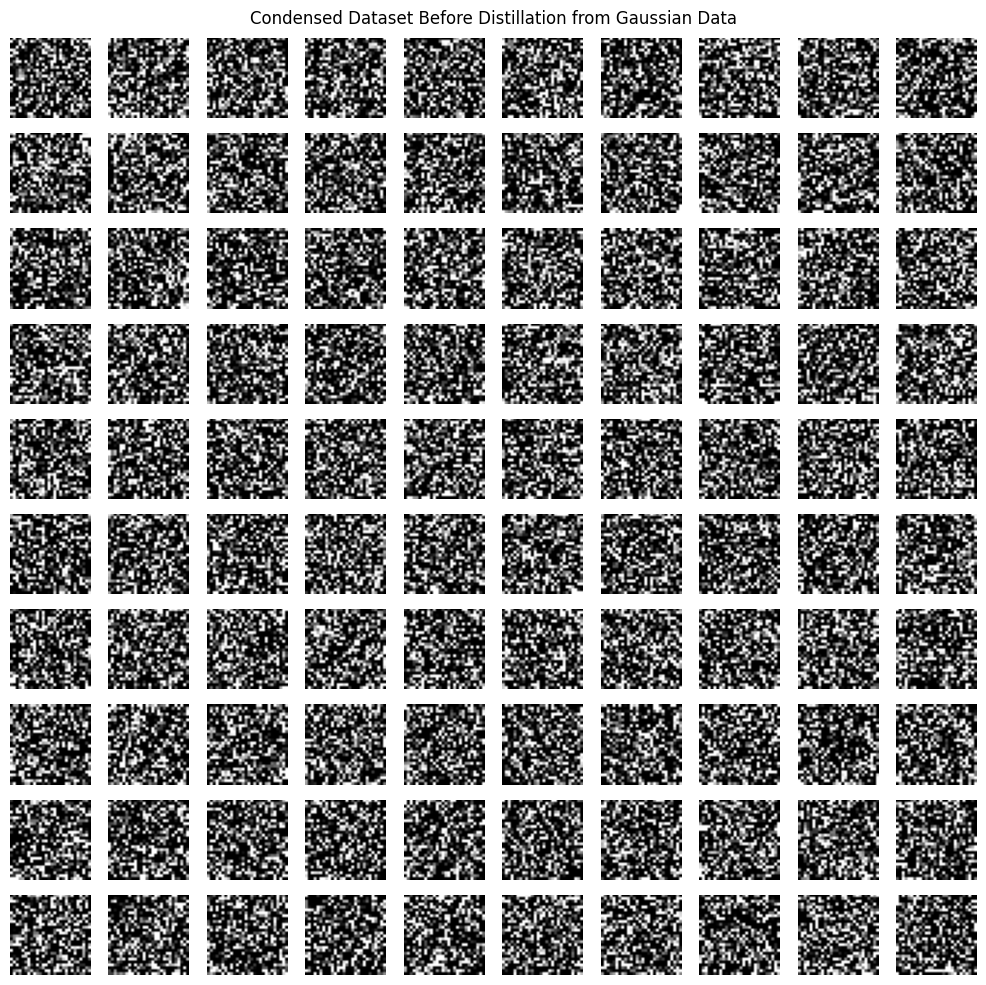
\includegraphics[width=0.95\textwidth]{images/MNIST_pad_before_distil_gaussian.png}
        \caption{The synthetic dataset before distillation from gaussian noise}
        \label{fig:MNIST_pad_before_distil_gaussian}
    \end{subfigure}%
    \begin{subfigure}{.5\textwidth}
        \centering
        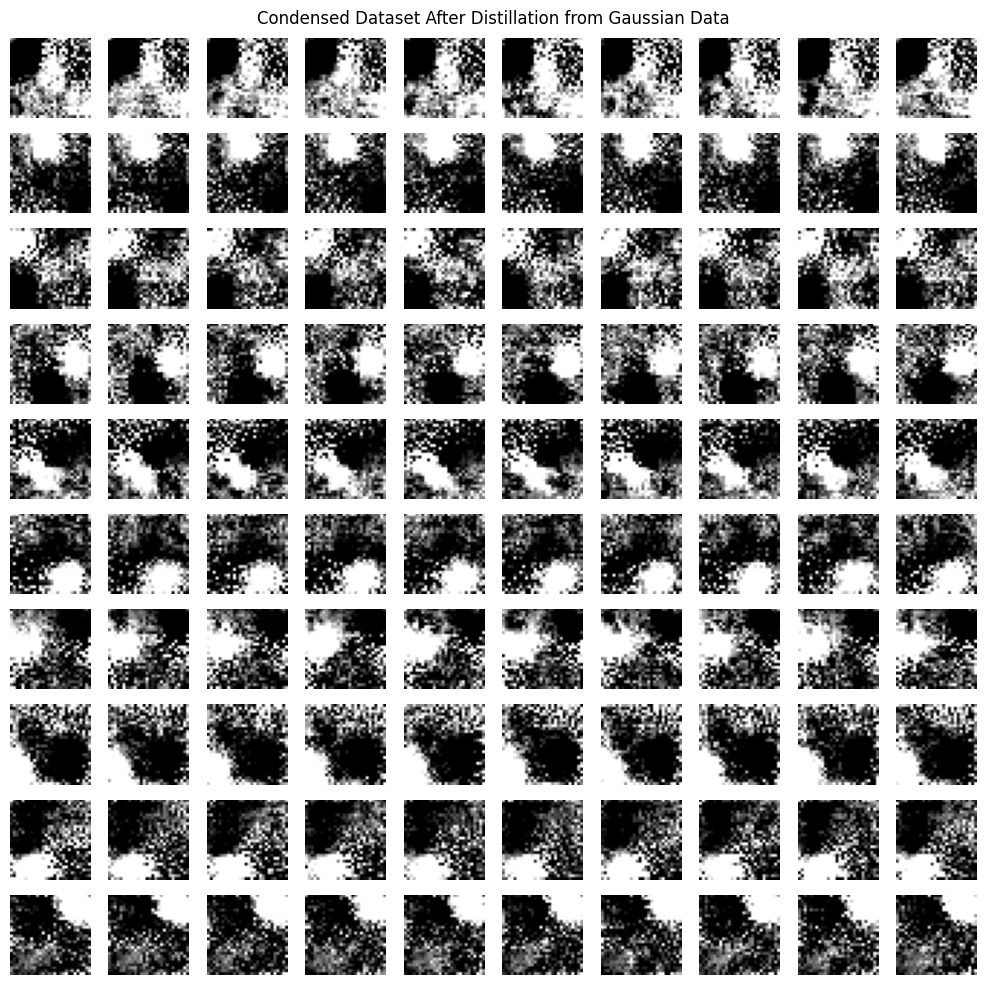
\includegraphics[width=0.95\textwidth]{images/MNIST_pad_after_distil_gaussian.png}
        \caption{The synthetic dataset after distillation from gaussian noise}
        \label{fig:MNIST_pad_after_distil_gaussian}
    \end{subfigure}
    \caption{The synthetic dataset before and after distillation from gaussian noise}
\end{figure}

Figure \ref{fig:MNIST_pad_before_distil_gaussian} displays the synthetic dataset before distillation from Gaussian noise, while Figure \ref{fig:MNIST_pad_after_distil_gaussian} shows the dataset after distillation. It is evident that the distillation method does not produce recognizable digits. As a result, we can anticipate poor performance when using this synthetic dataset to train a model.
\\
\subsubsection{Resutls and discussion for the MNIST dataset}
We then trained a ConvNet3D model for 50 epochs on the full MNIST dataset and on the two synthetic datasets. The results are shown in Table \ref{tab:MNIST_pad_results}.

\begin{table}[H]
    \centering
    \begin{tabular}{|c|c|c|c|}
        \hline
        Dataset & Full & From gaussian & From real \\
        \hline
        Accuracy & $99.43\%$ & $7.47\%$ & $68.62\%$ \\
        \hline
        Training Time & 7 min 32 s & $<$ 1 s & $<$ 1 s \\
        \hline
    \end{tabular}
    \caption{Results for the MNIST dataset}
    \label{tab:MNIST_pad_results}
\end{table}

The model trained on the real dataset achieved the highest accuracy; however, it required significantly longer training times compared to the synthetic datasets. The model trained on the synthetic dataset derived from Gaussian noise exhibited very low accuracy, which was expected given the quality of that dataset. In contrast, the model trained on the synthetic dataset distilled from real data demonstrated acceptable accuracy, making it a suitable choice for further tasks.
\\
Next, we evaluate the datasets in a cross-architecture setup by training AlexNet on the full MNIST dataset as well as on the two synthetic datasets. The results, shown in Table \ref{tab:MNIST_pad_results_cross_architecture}, indicate that the cross-architecture performance is poor on the synthetic datasets. This may be due to the fact that the synthetic dataset was generated using the specific characteristics of a ConvNet3D model, which AlexNet may not be able to effectively interpret.

\begin{table}[H]
    \centering
    \begin{tabular}{|c|c|c|c|}
        \hline
        Dataset & Full & From gaussian & From real \\
        \hline
        Accuracy & $99.15\%$ & $4.68\%$ & $13.68\%$ \\
        \hline
        Training Time & 8 min 24 s & $<$ 1 s & $<$ 1 s \\
        \hline
    \end{tabular}
    \caption{Results for the MNIST dataset on cross-architecture setup (AlexNet)}
    \label{tab:MNIST_pad_results_cross_architecture}
\end{table}

\subsubsection{Distillation of the MHIST dataset from real data}
To generate the synthetic dataset associated with the MHIST dataset, we used the PAD class. The parameters used were : $model = ConvNet7D$, $IPC = 50$, $K=200$, $T=10$, $\eta_S = 1$, $\zeta_S = 1$, $\eta_\theta = 0.01$, $\zeta_\theta=50$ and $\alpha=0.5$ (we take the data from all the layer as they are too few in ConvNet7D).

\begin{figure}[H]
    \centering
    \begin{subfigure}{.5\textwidth}
        \centering
        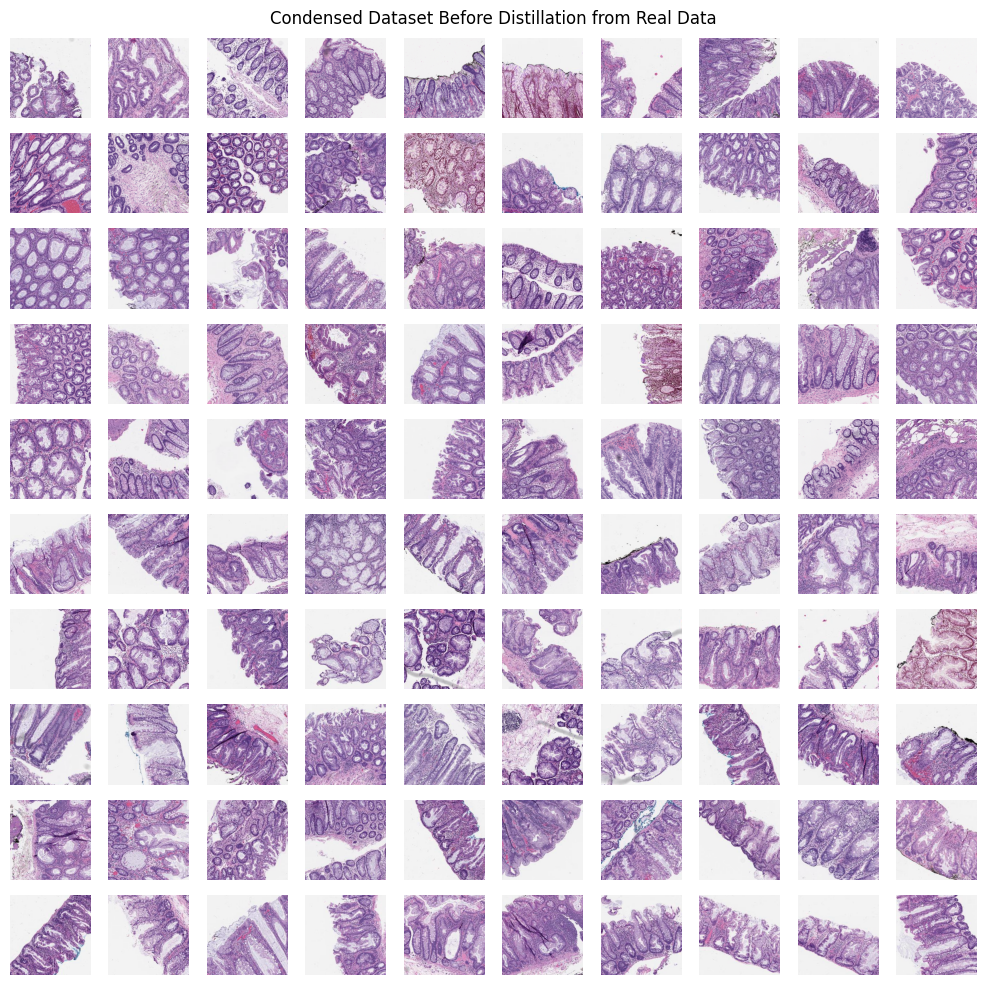
\includegraphics[width=0.95\textwidth]{images/MHIST_pad_before_distil_real.png}
        \caption{The synthetic dataset before distillation from real data}
        \label{fig:MHIST_pad_before_distil_real}
    \end{subfigure}%
    \begin{subfigure}{.5\textwidth}
        \centering
        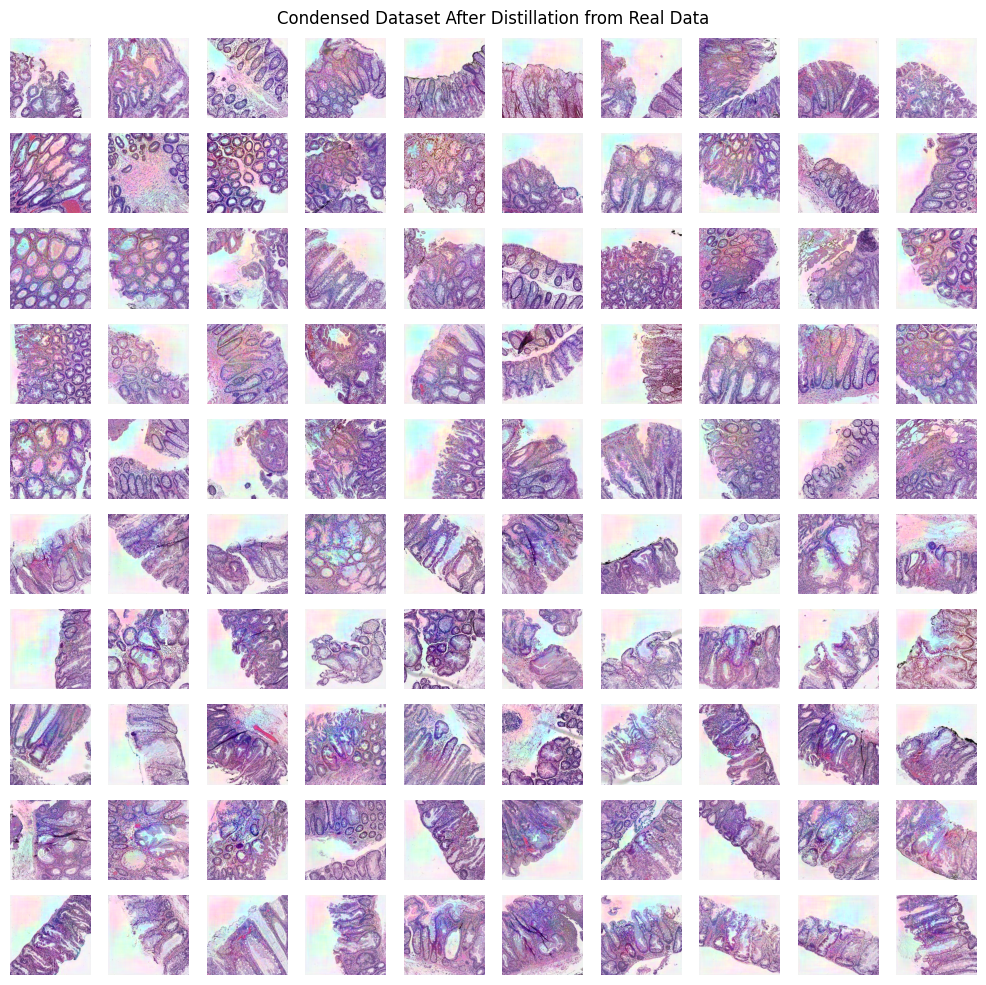
\includegraphics[width=0.95\textwidth]{images/MHIST_pad_after_distil_real.png}
        \caption{The synthetic dataset after distillation from real data}
        \label{fig:MHIST_pad_after_distil_real}
    \end{subfigure}
    \caption{The synthetic dataset before and after distillation from real data}
\end{figure}
Figure \ref{fig:MHIST_pad_before_distil_real} presents the synthetic dataset before distillation from real data, while Figure \ref{fig:MHIST_pad_after_distil_real} displays the dataset after distillation. At first glance, the synthetic dataset appears nearly identical to the real dataset, with the main differences observable in the backgrounds of the images. For a clearer understanding of the distinctions between the two datasets, we can refer to Figure \ref{fig:MHIST_2_diff_real}, which highlights the differences between the synthetic dataset before and after distillation. This figure demonstrates that the entire image is updated, indicating that the synthetic dataset is not merely a copy of the real dataset.

\begin{figure}[H]
    \centering
    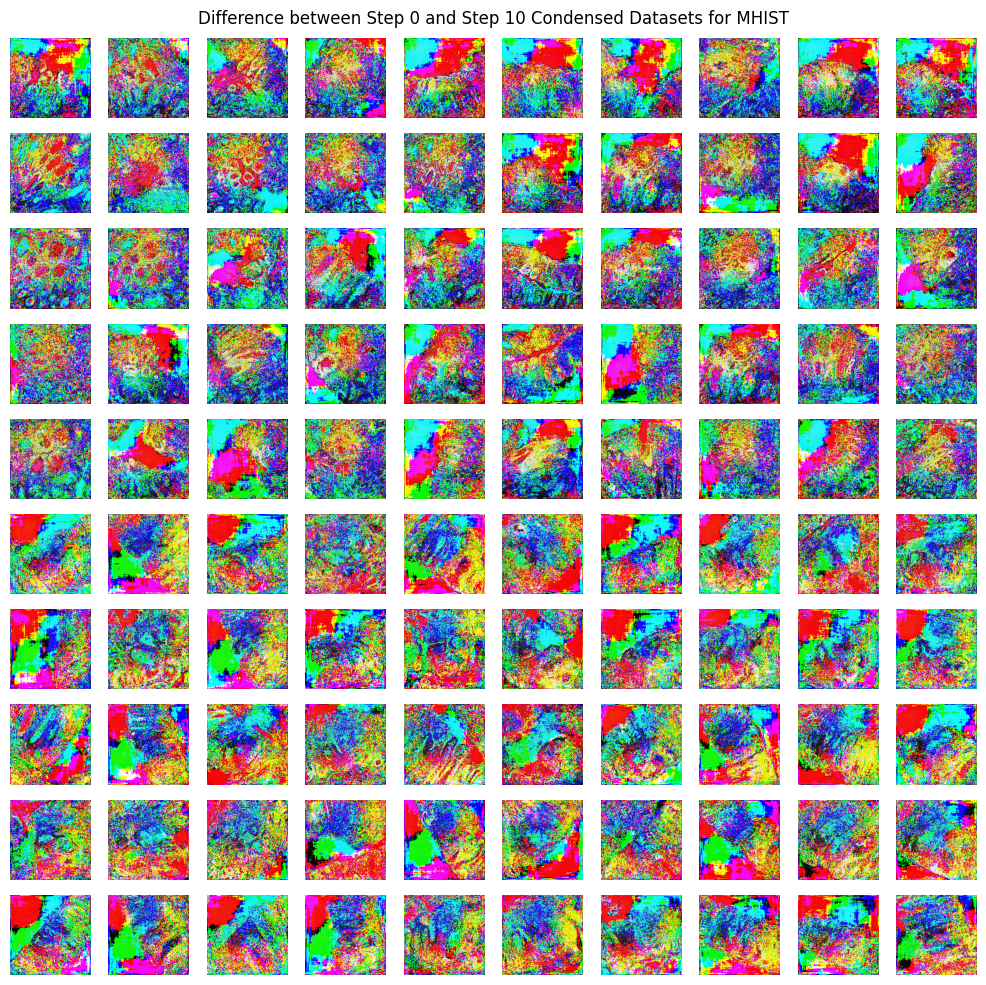
\includegraphics[width=0.5\textwidth]{images/MHIST_2_diff_real.png}
    \caption{The difference between the synthetic dataset before and after distillation from real data}
    \label{fig:MHIST_2_diff_real}
\end{figure}

\subsubsection{Distillation of the MHIST dataset from gaussian noise}
To generate the gaussin noise, we used a standard normal distribution. The parameters used were the same as for the distillation from real data except for $\eta_S = 10$.

\begin{figure}[H]
    \centering
    \begin{subfigure}{.5\textwidth}
        \centering
        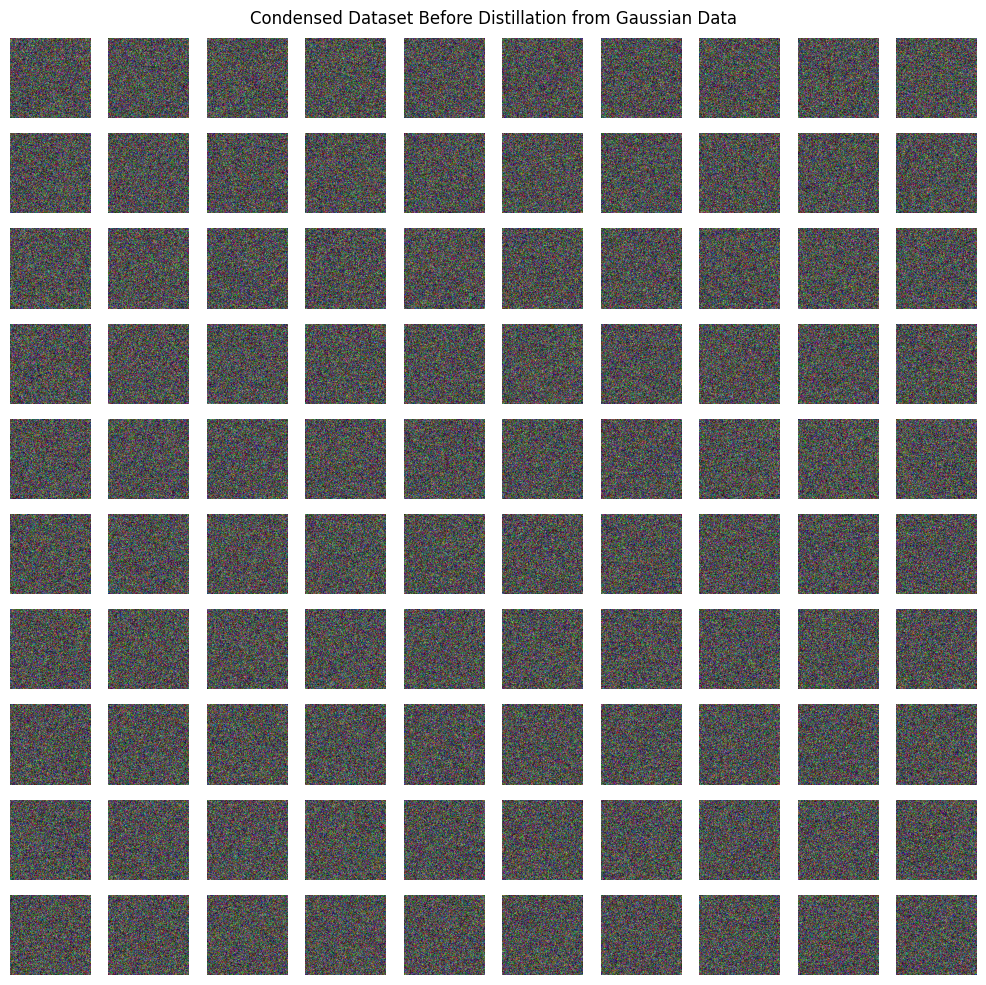
\includegraphics[width=0.95\textwidth]{images/MHIST_pad_before_distil_gaussian.png}
        \caption{The synthetic dataset before distillation from gaussian noise}
        \label{fig:MHIST_pad_before_distil_gaussian}
    \end{subfigure}%
    \begin{subfigure}{.5\textwidth}
        \centering
        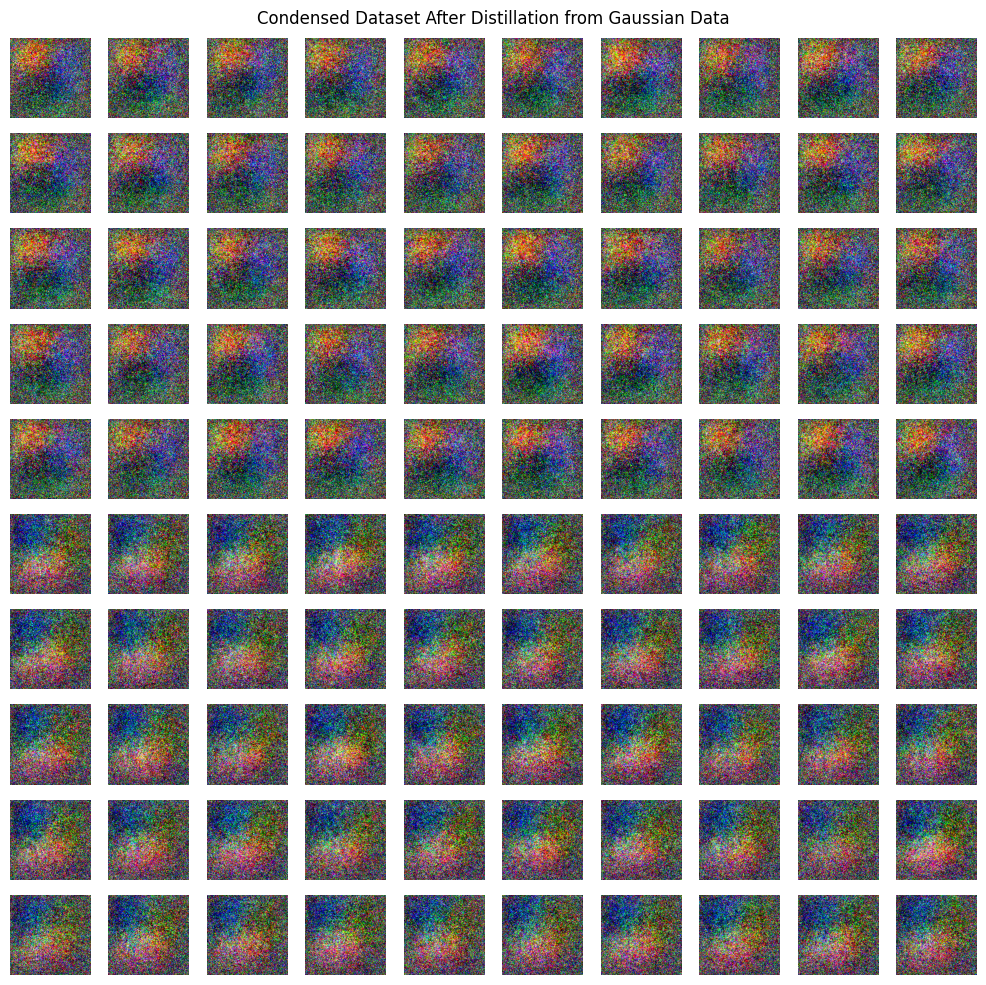
\includegraphics[width=0.95\textwidth]{images/MHIST_pad_after_distil_gaussian.png}
        \caption{The synthetic dataset after distillation from gaussian noise}
        \label{fig:MHIST_pad_after_distil_gaussian}
    \end{subfigure}
    \caption{The synthetic dataset before and after distillation from gaussian noise}
\end{figure}

Figure \ref{fig:MHIST_pad_before_distil_gaussian} displays the synthetic dataset before distillation from Gaussian noise, while Figure \ref{fig:MHIST_pad_after_distil_gaussian} shows the dataset after distillation. It is evident that the distillation method fails to produce recognizable shapes. Consequently, we can anticipate poor performance when using this synthetic dataset to train a model.
\\
\subsubsection{Resutls and discussion for the MHIST dataset}
\label{sec:MHIST_results_2}
We then trained a ConvNet7D model for 50 epochs on the full MHIST dataset and on the two synthetic datasets. The results are shown in Table \ref{tab:MNIST_pad_results}.

\begin{table}[H]
    \centering
    \begin{tabular}{|c|c|c|c|}
        \hline
        Dataset & Full & From gaussian & From real \\
        \hline
        Accuracy & $80.59\%$ & $54.65\%$ & $55.37\%$ \\
        \hline
        Training Time & 3 min 45 s & $<$ 8 s & $<$ 8 s \\
        \hline
    \end{tabular}
    \caption{Results for the MHIST dataset}
    \label{tab:MHIST_pad_results}
\end{table}

The model trained on the real dataset achieves the highest accuracy; however, it also requires longer training times compared to the synthetic datasets. Both models trained on the synthetic datasets exhibit low accuracy. While this is expected for the synthetic dataset derived from Gaussian noise, the synthetic dataset distilled from real data also demonstrates low accuracy, despite appearing visually correct. This could be attributed to the increased complexity of color images, which have three channels, making them more challenging to distill than grayscale images. Consequently, the model must learn more complex features due to the threefold increase in information to process.

Next, we evaluate the datasets in a cross-architecture setup by training AlexNet on the full MHIST dataset and on the two synthetic datasets. The results are shown in Table \ref{tab:MHIST_pad_results_cross_architecture}. Surprisingly, whereas cross-architecture performance was poor on the MNIST dataset, the models trained on the synthetic dataset using AlexNet achieve accuracy levels close to those of the models trained with ConvNet7D. This may indicate that, due to their subpar performance with ConvNet7D, the synthetic datasets are not specialized for that architecture and thus generalize better to a different architecture.

\begin{table}[H]
    \centering
    \begin{tabular}{|c|c|c|c|}
        \hline
        Dataset & Full & From gaussian & From real \\
        \hline
        Accuracy & $68.98\%$ & $55.785\%$ & $54.04\%$ \\
        \hline
        Training Time & 6 min 41 s & 18 s & 18 s \\
        \hline
    \end{tabular}
    \caption{Results for the MHIST dataset on cross-architecture setup (AlexNet)}
    \label{tab:MHIST_pad_results_cross_architecture}
\end{table}

\subsubsection{Neural architecture search}

We propose using the synthetic dataset to conduct a neural architecture search (NAS) aimed at identifying the best ConvNet model for classifying either the MNIST or the MHIST dataset. The search will encompass the following models: ConvNetD1, ConvNetD2, ConvNetD3, ConvNetD4, ConvNetD5, ConvNetW32, ConvNetW64, ConvNetW128, ConvNetW256, ConvNetAS, ConvNetAR, ConvNetAL, ConvNetASwish, ConvNetASwishBN, ConvNetNN, ConvNetBN, ConvNetLN, ConvNetIN, ConvNetGN, ConvNetNP, ConvNetMP, and ConvNetAP.
\\
The results for the MNIST dataset are shown in Table \ref{tab:NAS_results_MNIST}. We observe that searching for the best architecture using the synthetic dataset is significantly faster than training the best architecture on the full dataset. Notably, even though the synthetic dataset derived from Gaussian noise performs poorly, the best model identified remains consistent with the one found using the real dataset.

\begin{table}[H]
    \centering
    \begin{tabular}{|c|c|c|c|}
        \hline
        Search & From Real & From Gaussian \\
        \hline
        Best Model & ConvNetD4 & ConvNetD4\\
        \hline
        Accuracy on best model trained with synthetic data & $79.04\%$ & $11.35\%$ \\
        \hline
        Research time & 35 s & 35 s \\
        \hline
        Accuracy on best model trained on full data & $99.51\%$ & $99.5\%$ \\
        \hline
        Training time on full data & 7 min 37 s & 7 min 36 s \\
        \hline
    \end{tabular}
    \caption{Results for the MNIST dataset}
    \label{tab:NAS_results_MNIST}
\end{table}

For the MHIST dataset, the results are presented in Table \ref{tab:NAS_results_MHIST}. We observe that searching for the best architecture using the synthetic dataset is significantly faster than training the best architecture on the full dataset. However, the model identified through the neural architecture search does not perform as well as the model trained on the full dataset, as discussed in part \ref{sec:MHIST_results_2}. This discrepancy may arise from the fact that, unlike the MNIST dataset, the synthetic dataset for MHIST does not yield satisfactory performance. Consequently, utilizing it for a neural architecture search is less effective, as it propagates the inherent errors of the synthetic dataset.

\begin{table}[H]
    \centering
    \begin{tabular}{|c|c|c|c|}
        \hline
        Search & From Real & From Gaussian \\
        \hline
        Best Model & ConvNetD1 & ConvNetLN\\
        \hline
        Accuracy on best model trained with synthetic data & $65.19\%$ & $63.05\%$ \\
        \hline
        Research time & 10 min 51 s & 10 min 51 s \\
        \hline
        Accuracy on best model trained on full data & $68.57\%$ & $63.05\%$ \\
        \hline
        Training time on full data & 3 min 16 s & 4 min \\
        \hline
    \end{tabular}
    \caption{Results for the MHIST dataset}
    \label{tab:NAS_results_MHIST}
\end{table}

\section{Conclusion}
In this report, we presented two methods for distilling a synthetic dataset from a real dataset: DataDAM and Pad. Our findings indicate that DataDAM consistently outperforms Pad on both the MNIST and MHIST datasets. Additionally, we observed that neither method excelled in cross-architecture settings, suggesting limitations in generalizability across different models. Finally, we demonstrated that synthetic datasets can be effectively utilized for neural architecture search, with the synthetic dataset derived from real data proving to be superior to that generated from Gaussian noise. These insights highlight the potential of DataDAM for producing high-quality synthetic datasets and underscore the importance of dataset quality in enhancing model performance.

\bibliographystyle{plain}
\bibliography{mybibliography}
\newpage
% \section{Annex}
% \subsection{DataDAM code}
% \label{sec:DataDAM_code}
% Code for the DataDAM class. Mainly inspired from \cite{githubGitHubDataDistillationDataDAM}.
% \lstinputlisting{../DataDAM.py}
% \subsection{PAD code}
% \label{sec:PAD_code}
% Code for the PAD class. Partly inspired from \cite{githubGitHubNUSHPCAILabPAD}.
% \lstinputlisting{../PAD.py}
\end{document}
